% \documentclass{WHUBachelor}% 选项 forprint: 交付打印时添加, 避免彩色链接字迹打印偏淡. 即使用下一行:
 \documentclass[forprint]{WHUBachelor}
  \lstset{ 
    basicstyle=\small,% 
    escapeinside=``,% 
    keywordstyle=\color{red} \bfseries,% \underbar,% 
    identifierstyle={},% 
    commentstyle=\color{blue},% 
    stringstyle=\ttfamily,% 
    %labelstyle=\tiny,% 
    breaklines=true,
    extendedchars=false,% 
    linewidth=\textwidth,% 
    numbers=left,% 
    numberstyle=\tiny \color{blue},% 
    frame=trbl% 
    }


\begin{document}
%%%%%%% 下面的内容, 据实填空.

\title{实验项目三:具有独立内核的操作系统的实现}
\Cschoolname{数据科学与计算机学院}          % 学院名
\Cmajor{计算机科学与技术}                  % 专业中文名
\StudentNumber{16337237} % 填写自己的学号
\author{王永锋}                            % 作者名字
\Csupervisor{凌应标}        %指导教师中文名、职称
\date{二〇一八年三月三十一日}                % 日期, 要注意和英文日期一致!!

%----------------------------------------------------------------------------
\pdfbookmark[0]{封面}{title}         % 封面页加到 pdf 书签
\maketitle
\frontmatter
\pagenumbering{Roman}              % 正文之前的页码用大写罗马字母编号.
%-----------------------------------------------------------------------------
% \include{includefile/frontmatter}    % 加入摘要, 申明.
%==========================把目录加入到书签==============================%%%%%%
\pdfbookmark[0]{目录}{toc}
\tableofcontents
\mainmatter %% 以下是正文

%%%%%%%%%%%%%%%%%%%%%%%%%%%%%%%%%%%%%%%%%%%%%%%%%%%%%%%%%%%%%%%%%%%%%%%%%%%%%%%%%%%%%
%【实验方案】包括:硬件或虚拟机配置方法、软件工具与作用、方案的思想、相关原理、程序流程、算法和数据结构、程序关键模块,结合代码与程序中的位置位置进行解释。不得抄袭,否则按作弊处理。
%【实验过程】包括:主要工具安装使用过程及截图结果、程序过程中的操作步骤、测试数据、输入及输出说明、遇到的问题及解决情况、关键功能或操作的截图结果。不得抄袭,否则按作弊处理。
%【实验总结】每人必需写一段,文字不少于500字,可以写心得体会、问题讨论与思考、新的设想、感言总结或提出建议等等。不得抄袭,否则按作弊处理。
%【参考文献】(如有要列出,包括网上资源)
%%%%%%%%%%%%%%%%%%%%%%%%%%%--------main matter-------%%%%%%%%%%%%%%%%%%%%%%%%%%%%%%%%%%%%
\chapter{实验目的及要求}

\section{实验目的}

\begin{enumerate}
  \item 把原来在引导扇区中实现的监控程序(内核)分离成一个独立的执行体,存放在其它扇区中,为“后来“扩展内核提供发展空间。
  \item 学习汇编与c混合编程技术,改写实验二的监控程序,扩展其命令处理能力,增加实现实验要求2中的部分或全部功能。
\end{enumerate}

\section{实验要求}

本次实验,要求需要完成以下目标:\\

\begin{itemize}
  \item 规定时间内单独完成实验。
  \item 实验三必须在实验二基础上进行,保留或扩展原有功能,实现部分新增功能。
  \item 监控程序以独立的可执行程序实现,并由引导程序加载进内存适当位星,内核获得控制权后开始显示必要的操作提示信息,实现若干命令,方便使用者(测试者)操作。
  \item 制作包含引导程序,监控程序和若干可加载并执行的用户程序组成的1.44M软盘映像。
  \item 在指定时间内,提交所有相关源程序文件和软盘映像文件,操作使用说明和实验报告。
  \item 实验报告格式不变,实验方案丶实验过程或心得体会中主要描述个人工作,必须有展示技术性的过程细节截图和说明。
\end{itemize}

\chapter{实验方案}

\section{实验工具和环境}

本次实验平台\footnote{部分参考\cite{于渊2009orange}}搭建在win10系统的linux子系统上,通过编写makefile文件,连接nasm,gcc编译工具,dd二进制文件覆写工具,与bochs,qemu虚拟机加载配置文件与镜像(具体工具链详见下\autoref{tab:tools})。

与前几次实验相比,这一次实验代码的规模大了很多,仅仅凭借脚本并不容易将一整个项目进行高效的编译。因此,这一次我使用的是makefile来帮助这个项目进行自动化建构,只编译修改过的文件,而不编译不变的文件,以这种方式,加快了项目编译的速度,同时也能保证项目中各个文件之间的依赖关系不被破坏。

\begin{table}[htp]
  \caption{本实验所使用的工具链}
  \centering
  \begin{tabular}{cc}
    \toprule
    软件名称 & 用途  \\
    \midrule
    bash & 一个命令行终端,可提供linux的一些命令与执行shell脚本 \\
    nasm & 将x86汇编文件编译成.bin二进制文件 \\
    gcc & 编译工具,将c编译成二进制文件 \\
    ld & gcc套件中包含的连接器,用于将多个可执行文件连接起来 \\
    make & gcc套件中的工具,用于执行makefile文件 \\
    dd & 将二进制文件的内容写进软盘镜像中  \\
    objdump & 对可执行文件或二进制文件进行反编译 \\
    hexdump & 以十六进制形式查看软盘镜像文件 \\
    bochs & 虚拟机,用于加载装有自定义引导程序的软盘,使用软件模拟,速度不稳定  \\
    bochsdbg & 调试工具,用于给装有自定义引导程序的软盘文件进行调试 \\
    qemu & 虚拟机,用于加载装有自定义程序的软盘,使用硬件模拟,速度稳定且较快 \\
    \bottomrule
  \end{tabular}
  \label{tab:tools}
\end{table}

\section{相关基础原理-gcc与nasm的混合编程}

\subsection{32位与16位汇编代码的理解}

在gcc和nasm结合实现混编的过程中,其实遇到了不少的问题。但我认为,一个最大的问题在于对\textbf{32位汇编代码},\textbf{16位汇编代码}的区别的理解,与CPU在16位实模式下读取操作数,地址的方式的理解。

首先定义32位汇编代码,我认为的32位汇编代码,是\textbf{指使用了32位的寄存器,或者指令中的立即数是32位的,或操作32位的地址和操作数的指令}。而对16位汇编代码,也有类似的定义。

但是,在没有任何指令前缀的情况下,其实无论是32位的汇编代码还是16位的汇编代码,在机器指令级别上其实是看不出区别的。

这里说明一下,32位汇编指令和16位的汇编指令有以下共同点:

\begin{itemize}
  \item 操作码相同,如无论是从栈中取32位地址做返回地址的retl,还是从栈中取16位地址的ret,机器码都是0xc3。
  \item 寄存器索引相同。对于公有的寄存器,如ax,索引该寄存器的数字与索引eax寄存器的数字在机器指令层面是一致的。
\end{itemize} 

而32位汇编指令和16位汇编指令的差异在前面定义的时候已经讲得很清楚了,他们的差异主要体现在能在机器指令上看到的立即数的长度不同,还有隐含的处理器对寄存器或栈操作的行为的不同。


\begin{figure}[htp]
  \centering
  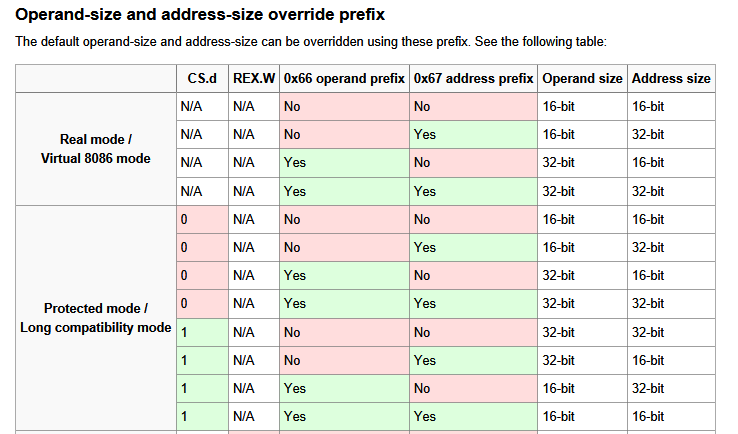
\includegraphics[width=12cm]{"./figure/wiki_prefix.png"}
  \caption{处理器在不同的模式下对指令的处理方式}
  \label{fig:wiki-prefix}
\end{figure}

当时想到这里,我就有一个特别特别严重的疑惑:从操作码上16位汇编指令和32位汇编指令完全相同,那么处理器自身是如何知道以何种方式(32/16)来处理这一些指令的呢?基于这样的疑惑,我在wiki上找到了这样的资料。

从这幅图中,可以看到,处理器处理指令的方式主要有两个因素来决定,一个是处理器当前所处模式,另一个是指令前缀的使用。\textbf{我们当前仍然处于16位实模式下,因此在没有任何前缀的情况下,处理器对指令的处理方式都是以16位的方式来进行处理的,而执行前若有0x66,0x67前缀,就意味着处理器在遇到这一条指令的时候,会使用32位的寄存器和操作数,或者处理指令中32位的地址。}

\subsection{实践中的验证}

之所以需要讲清楚32位汇编代码的共同点和差异点,是因为我们必须理解gcc生成的32位汇编代码与nasm产生的16位汇编代码之间的关系,同时认清CPU如何识别gcc生成的32位汇编代码,在理解的基础上,我们才能够有底气的使用这些工具给我们提供的各种功能,实现C与汇编交叉编译。

nasm 在使用bits 16 伪指令后,它能够生成16位的汇编指令,这些汇编指令有以下特点。

\begin{itemize}
  \item 操作码前没有前缀,处理器按16位实模式下默认方式工作。
  \item 指令长度较短,指令中的立即数长16比特,call指令中的偏移量长16比特。
  \item 在对栈进行操作的时候,push指令会把16位的操作数push进栈中。
  \item 操作的寄存器都是16位的。
\end{itemize}

gcc 在使用 -m16 选项编译后,他能够生成16位实模式下兼容的32位汇编指令,这些汇编指令有以下特点。

\begin{itemize}
  \item 操作码有前缀 0x66 或 0x67,表明处理器按照非默认方式(32位)读取操作数和地址。
  \item 指令长度较长,指令中的立即数长32比特,call指令中的偏移量长32比特。
  \item 对栈进行操作的时候,push指令会把32位的操作数push进栈中。
  \item 操作32位的寄存器(如eax等)
\end{itemize}

这些指令在机器代码上的区别可见图\autoref{fig:nasm-16asm},\autoref{fig:gcc-32asm}。

\begin{figure}[htp]
  \centering
  \begin{minipage}[t]{0.5\linewidth} 
  \centering
  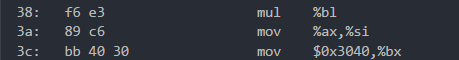
\includegraphics[width=10cm]{"./figure/nasm_16asm.png"}
  \caption{nasm生成的16位汇编代码}
  \label{fig:nasm-16asm}
  \end{minipage}

  \begin{minipage}[t]{0.5\linewidth} 
  \centering
  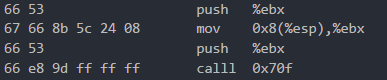
\includegraphics[width=10cm]{"./figure/gcc_32asm.png"}
  \caption{gcc生成的32位汇编代码}
  \label{fig:gcc-32asm}
  \end{minipage}
\end{figure}

在这里,我们证实了以下两个结论:

\begin{itemize}
  \item 无论是gcc,还是nasm,只要使用恰当的编译指令产生的机器指令,都能够在16位实模式下正确运行。
  \item nasm与gcc产生的汇编代码,在相互调用的时候可能会产生问题,问题主要在c的call是push32位地址,而nasm的ret是取16位地址。一来一回就会产生问题。
\end{itemize}

\subsection{gcc和nasm产生可执行文件的可连接性}

上面证实了指令的可运行性,这里在确认一下两种可执行文件的可连接性。

要保证两种可执行文件可以连接,必须保证两种文件有着相同的可执行文件的格式。所幸,通过搜寻资料,我发现nasm在使用-f elf32的情况下能够输出elf32格式的可执行文件,gcc在-m16的默认情况下输出一种格式为elf32的可执行文件,同时,连接器也支持使用-m elf\_i386的指令,连接两个elf32格式的可执行文件,这就为最终连接成功奠定了基石。

同时,考虑到最终生成的可执行文件还不能直接写入软盘,我们还需要生成不包含文件头的纯二进制文件,对于这个需求,ld工具中控制输出格式的一个参数--oformat binary可以用来控制输出文件的格式。

以下是编译指令样例

\begin{lstlisting}
  nasm -f elf32 -o kernel.o kernel.asm
  gcc -c -m16 -ffreestanding -o start.o start.asm
  ld -Ttext 0x00000 -m elf_i386 --oformat binary -o kernel.bin kernel.o start.o
\end{lstlisting}

在上面有两个指令没有说明的,一个是gcc中的-ffreestanding ,这个指令的用途是表明这个程序没有用到任何库函数,不能够对库函数做优化;另一个是 ld工具的-Ttext 0x00000 ,他的作用与org类似。

同时,还有一个显而易见不需要说明的是,代码中必须有global,extern等关键词用作将名字导出或导入,这样之后的连接器才能够正确识别并连接。不过,由于elf格式的特殊性,名字在编译后不会产生下划线前缀(NASM文档中有提到)

至此,C与汇编混合编程完成。

\subsection{gcc和nasm下c与汇编混合编程的方法}

在证实指令的运行性和可连接性后,对两个不同的编译器产生的有一点点相互不兼容的地方,我们做以下妥协,保证代码的正确运行。

\begin{itemize}
  \item 为确保统一,代码中出现的call和ret统一显式指明使用32位格式。具体的方式是:
  \begin{lstlisting}[language={[x86masm]Assembler}]
    ; 使用宏,在ret指令前显式添加0x66前缀
    %macro retl 0
    db 0x66
    ret
    %endmacro
    ; 在call的时候添加 dword,确保call产生32位的偏移量。
    call dword LABEL
  \end{lstlisting}

  \item gcc生成汇编代码的过程中,可能会生成用到段寄存器的指令(如从数据段获取数据)。这里我们需要了解gcc一般会默认cs,ss,ds,es等段寄存器都是一致的。因此在跳入C代码段的时候,要确保段寄存器的一致性。

  \item gcc遵循C调用约定,因此关于参数传递以及返回值的规范需要汇编代码遵守。
  
\end{itemize}

\section{程序功能说明及大致思路阐述}

这里会对程序的大致运行流程进行一个粗略的描述,同时罗列了当前系统内核支持的功能。

\subsection{程序大致思路阐述}

\begin{enumerate}
  \item 一开机,处于软盘第一个扇区的引导程序加载第72-89个扇区,作为系统内核,并将控制权转交给系统内核。
  \item 系统内核刚开始运行,经过一系列初始化工作(如安装中断,加载fat表,根目录表),跳转到tty例程(即用户终端。
  \item 进入到命令行中断,系统管理员可以在这里执行一系列指令 TODO:
\end{enumerate}

\subsection{程序功能说明}
TODO:对程序功能需要进一步完善。
本程序(完整程序代码见附件)实现了以下功能(主界面可见\autoref{fig:main_screen})。
\begin{enumerate}
  \item \textbf{按下1。}
\end{enumerate}

\section{代码框架的设计}

\subsection{库文件说明}

为了能够在C中更有效的操作硬件,同时保证更有效率的开发,我实现了以下库函数作为内核需要调用的头文件。对于一些无法使用C语言实现的功能,如端口的读写,我使用汇编语言实现了一些函数,将端口读写封装成一个个C语言直接可用的函数,而对bios中断的使用也是类似,在basic.asm中实现了对一些bios中断的直接调用,那么在C中,就可以对这些硬件操作进行进一步的封装(主要在stdio.c中实现),实现一些对开发者友好的接口,从而加快开发操作系统的效率。

\begin{table}[htp]
  \caption{库文件说明}
  \centering
  \rowcolors{1}{White}{Lavender}
  \begin{tabular}{lp{11cm}}
    \toprule
    头文件名 & 功能说明 \\
    \midrule
    basic.asm & 实现一些只能通过汇编实现的接口函数 \\
    stdio.c & 存放处理I/O的函数(如printf) \\
    system\_call.c & 用于存放各项系统调用(暂时只写了安装系统中断) \\
    string.c & 用于字符串的处理,包括比较和复制等函数 \\
    global.c & 存放全局变量(目前有系统调用表) \\
    fsystem.c & 存放负责处理文件的函数 \\
    \bottomrule
    \hiderowcolors
  \end{tabular}
  \label{tab:library}
\end{table}

\subsection{命令行终端的实现}

命令行终端主要在tty.c中实现,该份代码的主要编写思路为:
\begin{itemize}
  \item 使用终端内的全局变量,作为输入缓冲区,显示位置,光标偏移量。每输入一个字符,根据缓冲区的内容以及其他变量刷新显示内容。
  \item 终端建立一个事件循环,一旦有字符键入,check\_keyboard()函数返回的值会让终端知道有字符键入,触发终端对这个事件的发生产生响应。
  \item 使用get\_keyboard()函数返回的值,判断键盘输入内容,从而进行对应事件的响应,如键入enter,会触发命令行的执行,键入可打印字符,会触发输入缓冲区的显示刷新。
  \item 一旦进入解析器,解析器会读取输入缓冲区的内容,进行分词,然后根据相应的参数调用对应的过程。
\end{itemize}



\subsection{命令行终端与文件系统的交互}

\begin{itemize}
  \item 运行程序的过程
  新建一个函数指针的指针,并且指明这个函数处在0x2000这个偏移量中,然后使用文件系统将相应的文件加载到对应地址,最后调用该函数实现跳转。
  \begin{lstlisting}[language=c]
   if(!strcmp(arguments[0],"run")){// 如果返回0,就是相等了
    void (**my_program)();
    *my_program = 0x2000;
    fs_load_by_name(arguments[1],*my_program);
    (*my_program)();
  }
  \end{lstlisting}
  \item 打印文件列表及信息,只需要直接调用文件系统提供的接口就行了。
  \begin{lstlisting}[language=c]
  if(!strcmp(arguments[0],"ls") && arguments_num == 1){
      printf("\n\n");
      fs_show_root_file_table();
  }
  \end{lstlisting}
\end{itemize}

\chapter{实验难点及亮点}

在完成本次实验的过程中,在下面的功能中花了比较长的时间,而且是在原有实验要求上所没有的,有一些即使在这一次实验中没有完全用上,也能够在之后的实验中继续用于完善操作系统。

\section{文件系统模块的实现}

在这一个操作系统中,文件系统模块主要由“fsystem.h”和“fsystem.c”来实现。
对于文件系统中所需要的读写格式,我在“fat.asm”和“root.asm”中进行编码然后写进硬盘中。

\subsection{总体原理概述}

\subsubsection{所需文件}

\begin{table}[htp]
  \caption{文件系统相关文件说明}
  \centering
  \rowcolors{1}{White}{Lavender}
  \begin{tabular}{lp{11cm}}
    \toprule
    文件名 & 功能说明 \\
    \midrule
    ./boot/fat.asm & 硬编码fat表,写入到软盘的第二个扇区 \\
    ./boot/root.asm & 硬编码根目录表,写入到软盘的第37个扇区 \\
    ./include/fsystem.h & 文件系统头文件,包含了文件系统操作的各类函数的声明 \\
    ./lib/fsystem.c & 文件系统代码文件,包含了文件系统操作的函数的实现 \\
    \bottomrule
    \hiderowcolors
  \end{tabular}
  \label{tab:library}
\end{table}

\subsubsection{文件系统实现功能}

\begin{enumerate}
  \item 向文件系统传入文件名尝试进行加载,加载成功的状态由返回的错误码来判断。
  \item 向文件系统传入文件名读取文件信息
  \item 向文件系统请求打印根目录文件信息
\end{enumerate}

\subsection{实现细节}

\subsubsection{软盘的抽象}

目前文件系统的实现中,唯一依赖的一个底层函数是定义在basic.c中的read\_sector()函数,这个函数是int13h中断的再包装。文件系统其余的函数只要涉及到软盘到内存的I/O操作,都需要用到这一个函数。基于这一个函数,在int 13h已有的抽象下,进一步将软盘抽象,从而只通过逻辑扇区号和扇区数量就可以直接加载对应的扇区。

基于以上的封装,我实现了以下函数,从而将软盘进一步抽象,从而能够通过文件名直接访问。

\begin{table}[htp]
  \caption{文件系统相关函数说明}
  \centering
  \rowcolors{1}{White}{Lavender}
  \begin{tabular}{lp{11cm}}
    \toprule
    函数声明及相关功能 \\
    \midrule
    u16 \_fs\_find\_descriptor\_number\_by\_name(char * file\_name);  \\
    内部过程:使用文件名,找到对应文件描述符的索引。 \\
    u16 \_fs\_find\_cluster\_code\_by\_name(char * file\_name); \\
    内部过程:使用文件名,找到该文件的簇号 \\
    u16 \_fs\_get\_file\_size\_by\_cluster\_code(u16 cluster\_code);  \\
    内部过程:从簇号,找到这一整个文件占用的空间大小 \\
    void \_fs\_show\_file\_by\_descriptor\_number(u16);  \\
    内部过程:使用文件描述符的索引,展示该文件信息 \\
    u16 \_fs\_load\_by\_cluster\_code(u16 first\_cluster\_code, void (*program)() );  \\
    内部过程:使用簇号,加载fat表中的一系列扇区到指定的地址处。 \\
    u16 fs\_load\_by\_name(char * file\_name, void (*program)());  \\
    对外过程:使用文件名,加载对应文件到指定地址处,返回错误码判断是否加载成功。 \\
    u16 fs\_get\_file\_size(char * file\_name);  \\
    对外过程:使用文件名获取文件大小(为之后分配内存做准备) \\
    void fs\_show\_file\_by\_name(char * file\_name);  \\
    对外过程:使用文件名,展示对应文件信息 \\
    void fs\_show\_root\_file\_table();  \\
    对外过程:打印文件目录表 \\
    \bottomrule
    \hiderowcolors
  \end{tabular}
  \label{tab:library}
\end{table}

\subsubsection{read\_n\_sector函数的实现}

这个函数作为文件系统与bios中断之间极其重要的抽象层,将需要磁头号,柱面号,扇区号访问的软盘,抽象成只通过从0开始的逻辑扇区号来访问,将软盘转变成一个像是数组的连续存储介质。同时,该函数还能够将指定数量扇区的内容加载到指定的地址中,从而完美封装了int 13h中断。以下是代码实现。

\begin{lstlisting}[language=c] 
/* tested
读取指定逻辑扇区号的扇区到指定内存地址处
注意一次最多写一个段,也就是64k 最多读128个扇区。*/
void read_n_sector(u16 sector_code, u16 number,  u16 segment, u16 offset){
    for (int i = 0; i < number; i++){
        int sector = (sector_code+i) % 18+1;
        int mid = (sector_code+i) / 18;
        int cylinder = mid >> 1;
        int head = mid & 1;
        read_sector(head, cylinder,sector,segment, offset + i*512);
    }
    return ;
}
\end{lstlisting}

\subsubsection{加载指定文件所需函数的实现}

为了实现通过文件名就可以加载指定文件到指定地址,我实现了两个子函数。

\begin{enumerate}
  \item 文件名->簇号
  \begin{lstlisting}[language=c] 
    u16 _fs_find_cluster_code_by_name(char * file_name){
      int index = _fs_find_descriptor_number_by_name(file_name);// 实现从文件名找到对应的文件描述符索引
      if (index != -1) // 若索引存在
          return root[index].cluster_code;
      return 0;
  }
  \end{lstlisting}
  \item 加载从指定簇号开始的一系列扇区(由fat表确定簇数量)到指定函数指针处。
  \begin{lstlisting}[language=c] 
  u16 _fs_load_by_cluster_code(u16 cluster_code, void(*program)()){
      int size = 0;
      while (0x0002 <= cluster_code && cluster_code <= 0xFFEF){
          size += 512*cluster2sector;
          int sector_number = first_cluster_by_sector + (cluster_code-2)*cluster2sector;
          read_n_sector(sector_number, cluster2sector, 0x1000, program);
          program = program+cluster2sector*512;
          cluster_code = FAT_table[cluster_code];
      }
      return size;
  }
  \end{lstlisting}
\end{enumerate}


\section{可自定制的中断系统-系统调用前奏}

总是看到dos能够通过下面代码所示的方式调用系统调用,在这里我自己也尝试了一些这样调用中断的实现。
\begin{lstlisting}[language={[x86masm]Assembler}]
  mov ax, 4c00h
  int 80h
\end{lstlisting}

\subsection{功能及原理说明}

这里我实现了这样的一个中断,内核可以在程序中以如下代码的方式安装中断:
\begin{lstlisting}[language=c]
  void test_system_call();
  int cstart(){
      install_system_call(2, test_system_call);
      // 将指定的函数安装到2号系统调用中
  }
  void test_system_call(){
      int origin = get_cursor();
      set_cursor(1800);
      printf("test custom system call!!! ");
      set_cursor(origin);
  }
\end{lstlisting}

然后在汇编中,我便可以用下面的方式直接调用我之前安装的系统调用测试函数!

\begin{lstlisting}[language={[x86masm]Assembler}]
  mov ax, 0x0200h
  int 40h
\end{lstlisting}

\subsection{实现原理}

在内核中,我维护着一个数组“系统调用表”,该数组存储着不同的系统调用的地址,在C语言中安装中断,就是将对应函数指针的内容,写到相应数字索引的系统调用表中。

而我自己的int 40h中断,则是先读入ah寄存器的内容,计算该系统调用的系统调用号的索引,然后在系统调用表中找到对应的表项并且call过去,运行完指定函数之后回来恢复现场,继续执行下面的代码。

同时,该中断也可通过功能号4c,实现子程序的返回,可返回到命令行终端模式。

详情可见\autoref{code:int_40h}

\section{原理清晰,结构合理的gcc-nasm编译工具链}

本次项目,重新组织了代码文件,对各个模块的整理,可见\autoref{code:organization}。

\subsection{各文件夹的作用}

\autoref{tab:folder}描述了各个文件夹的作用

\begin{table}[htp]
  \caption{文件夹的说明}
  \centering
  \rowcolors{1}{White}{Lavender}
  \begin{tabular}{lp{11cm}}
    \toprule
    文件夹名称 & 文件夹用途 \\
    \midrule
    boot & 里面包含了引导扇区的汇编代码,以及需要硬编码到软盘的文件系统相关数据 \\
    kernel & 里面包含了内核代码及命令行终端的实现 \\
    include & 这里是库文件的头文件,主要用作各种函数的引用 \\
    lib & 里面有各个库文件的定义,需要和用到这些函数的文件一起编译 \\
    user & 里面存放了各个用户程序 \\
    \bottomrule
    \hiderowcolors
  \end{tabular}
  \label{tab:folder}
\end{table}

\subsection{编译工作的进行}

在os文件夹下具有一个主makefile文件,这个文件先进入到各个子文件夹进行building,构建各个模块的二进制文件,再回到这个主makefile文件进行将二进制文件写入到软盘的工作,并且集成了各个工具的使用,直接打开虚拟机查看结果。

\chapter{曾经遇到的问题}

\section{读端口的函数没有返回值}

在C调用约定中,有一条这样的约定:返回值使用ax寄存器返回。在实现读端口数值的时候,我犯了这样一个愚蠢的错误,在保存寄存器的时候误把ax作为一个被调用者保存寄存器保存起来,导致返回值无法传递到调用者,代码如下所示:

\begin{lstlisting}[language={[x86masm]Assembler}] 
  ; tested 从8位端口读出8位的值
  ; u8 read_port_byte(u16 port_number);
  read_port_byte:
  push ebp
  mov ebp, esp
  push dx
  push ax ; !!!不能保存ax寄存器的值,要作为返回值传递给调用者
  ;enter
  mov dx, [ebp+8]  ; 取第一个参数  端口号
  in  al, dx
  ;laeve
  pop ax ; !!!
  pop dx
  mov esp, ebp
  pop ebp
  retl
\end{lstlisting}

相同的错误在其他地方也出现过多次,就不再赘述。

\section{无法正常的获取光标位置}

在获取光标位置的函数中,无法获取光标的位置。主要的原因是以下代码出现错误,导致光标索引计算错误!

\begin{lstlisting}[language={[x86masm]Assembler}] 
  cursor_index = cursor_index << 8 + low_eight;
\end{lstlisting}
事实上,+号的优先级比移位高,我需要加一个括号,像下面一样才能正常运行。
\begin{lstlisting}[language={[x86masm]Assembler}] 
  cursor_index = (cursor_index << 8) + low_eight;
\end{lstlisting}

\section{printf函数的实现}

在实现printf函数的过程中,经历了内存被神秘改写的奇特bug,经过细细调试,定位这样的问题:栈指针初始化的不合理,导致栈段与代码段重合。

在开发的时候会有开发日志记录自己在开发过程中遇到的问题,下面从这个bug的解决中摘录一部分。\autoref{fig:printf_bug}

\begin{figure}[htp]
  \centering
  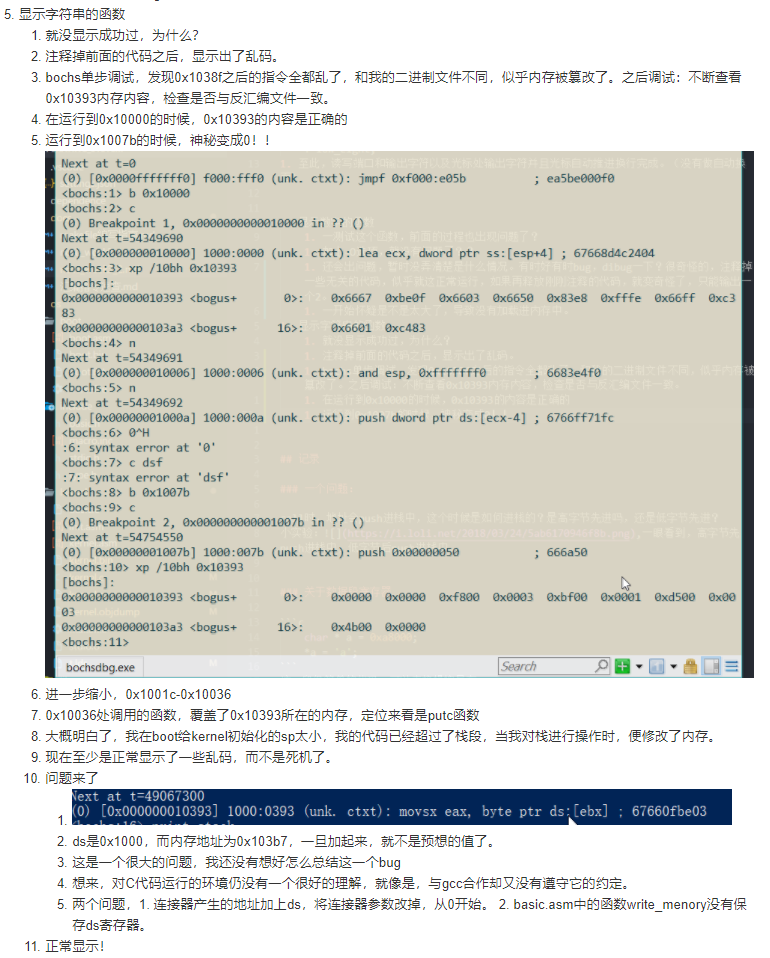
\includegraphics[width=18cm]{"./figure/printf_bug.png"}
  \caption{printf函数-开发日志摘录}
  \label{fig:printf_bug}
\end{figure}

\section{对段寄存器在C程序中起的作用的理解}

\begin{lstlisting}[language=c]
  char * a = 0xa8000;
  *a = 'a';
\end{lstlisting}
  
  这一段很简单的代码,可以直接操控显存。
  为什么不是B8000呢,因为我的ds被初始化为0x1000了。
  这也是段寄存器在c语言中起作用的典型例子,之前一直没搞清楚c语言中段寄存器如何起作用。
  在使用bochs调试的时候,通过反汇编,看到了这条语句在寻址过程中对指针的使用。
  
\section{在实现文件系统前遇见的bug}

在运行的时候,发现如果我注释掉一段代码,就会让程序正常运行,如果我恢复那一段代码,程序就会进入一种不正常的运行状态,一些应该显示的信息没有显示出来。后来发现,是内核的大小超出了加载的扇区数量,这也是后来我想做文件系统的动机之一。

\autoref{fig:user_bug}摘录自开发日志。

\begin{figure}[htp]
  \centering
  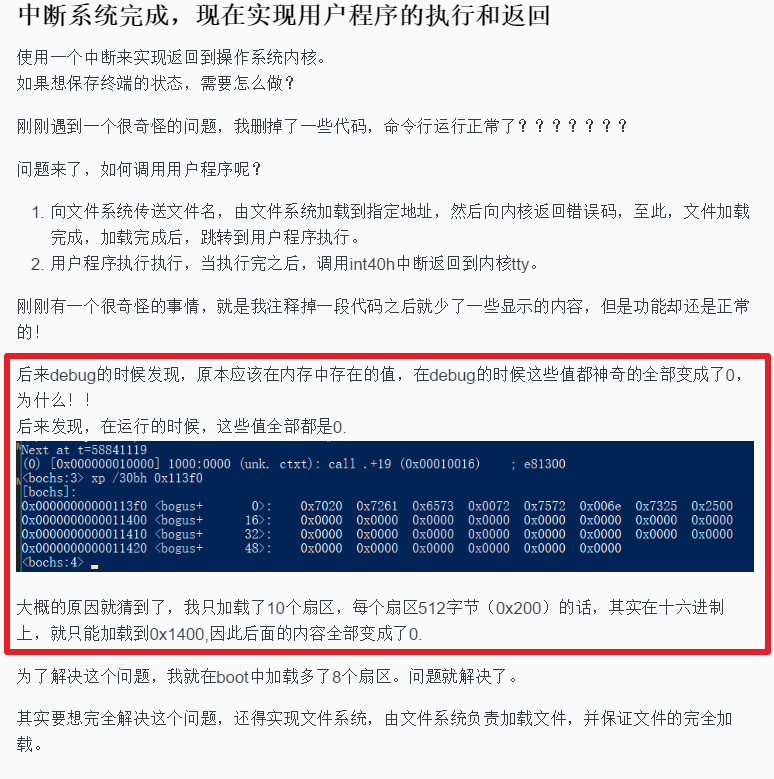
\includegraphics[width=17cm]{"./figure/user_bug.png"}
  \caption{user用户程序-开发日志摘录}
  \label{fig:user_bug}
\end{figure}


\chapter{实验结果}




\section{命令行终端的测试}

TODO:功能的展示。
本程序经nasm,gcc编译后在qemu虚拟机下运行的效果可见\autoref{fig:main_screen}与\autoref{fig:main_screen2},其中\autoref{fig:main_screen2}中的边框可以逆时钟旋转同时随机地改变颜色。
\begin{figure}[htp]
  \centering
  \begin{minipage}[t]{0.5\linewidth} 
    \centering
  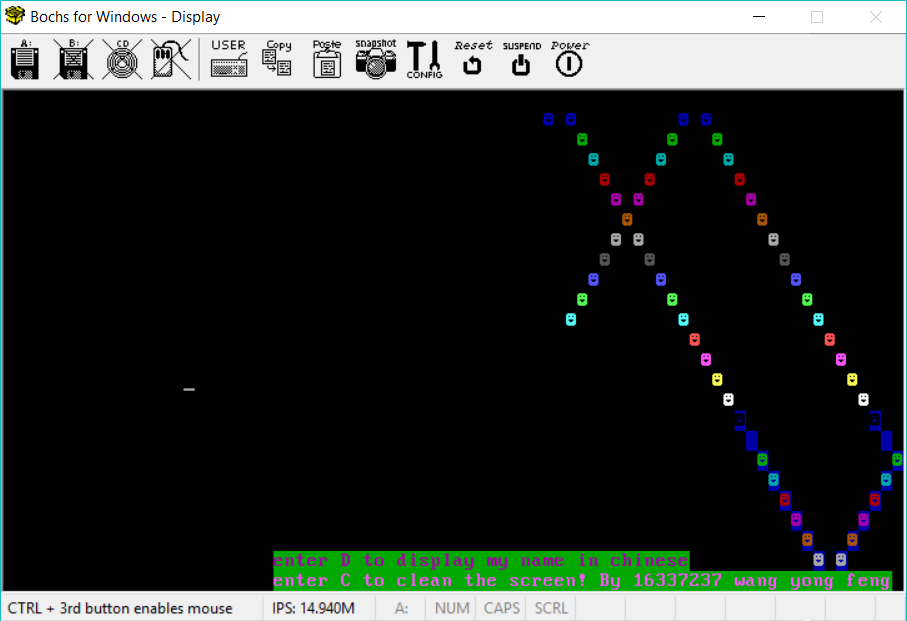
\includegraphics[width=10cm]{"./figure/main_screen.png"}
  \caption{命令行终端的主界面}
  \label{fig:main_screen}
\end{minipage}

  \begin{minipage}[t]{0.5\linewidth} 
  \centering
  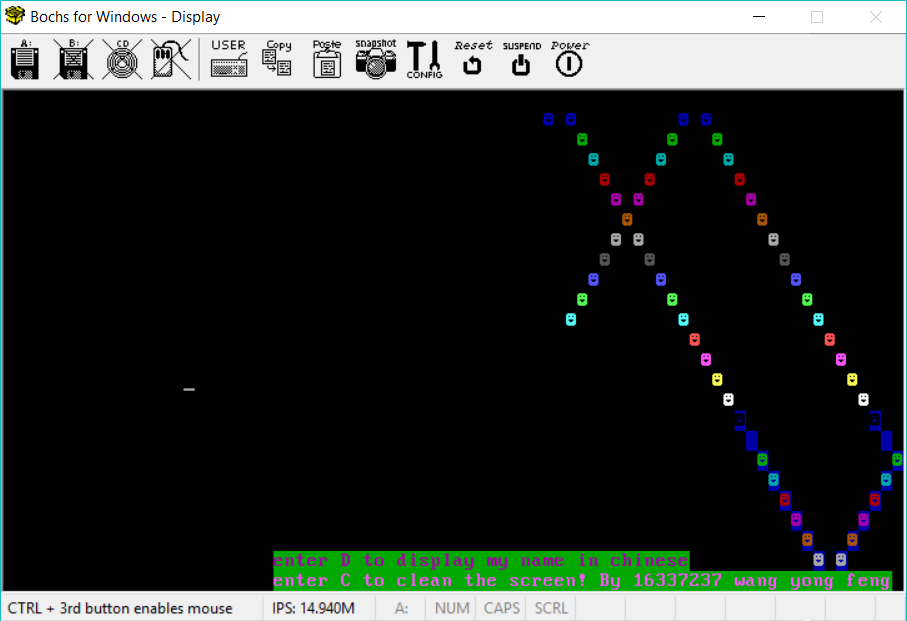
\includegraphics[width=10cm]{"./figure/main_screen.png"}
  \caption{自定义引导程序按下D后的界面}
  \label{fig:main_screen2}
\end{minipage}
\end{figure}

\section{自定义系统调用的测试}

TODO:

\section{文件系统的测试}

TODO:

\chapter{实验总结}

这是实验三的实验总结。

在实验前期,我对c与汇编混合编程的概念并不了解。在一开始接触到混合编程的时候,甚至是想了半天为什么要使用c语言和汇编混合编程,还想了很久需要使用C语言做什么事情,紧接着,对C语言中隐藏的细节再进行了很多的思考,以想明白如何使用c语言替换汇编的代码。

C语言,可以说是已经很贴近硬件底层的语言了,可是直到我将C语言与汇编语言结合起来使用,我才更进一步的认识到C语言对内存的操控能力。在C中,我可以对地址进行直接的操作,使用指针的方式,修改特定位置的内存的数据。同时,通过修改函数指针,我们甚至可以修改ip,从而达到在汇编中与call一致的效果。

但同时,C语言也对我们隐藏了很多硬件的细节,也正是这些细节,让我在一开始觉得C语言的行为有一些不可控的因素。其中一个很重要的点就是寄存器的使用,在C中,我们不会也不能对寄存器进行直接的操作,我们创建的所有变量要么是编译器决定使用寄存器,要么是使用用户的栈空间申请一些临时变量,这一切的细节,都由编译器来完成,而我们无需关心具体寄存器还是栈,我们只需要关心数据的处理与使用就可以了。从这个角度上来讲,使用C语言也更能让我们在硬件的众多细节中脱身而出,让我们有更多的精力去关注代码中的逻辑与功能。

C语言对我们隐藏的另一个细节是段寄存器的使用。C语言中,无论我们怎么写代码,其实都是默认在一个段中,而显然编译器也是这么认为的。编译器会直接拿C语言汇编出来之后的汇编地址放到代码中需要地址的地方,然后在访问的时候按照处理器的规则,加上ds或者cs去访问。

对段寄存器细节的隐藏,一方面是解脱了一些细节的纠缠,但另一方面,却让我的代码的组织变得有些困难。我当然可以整个操作系统只使用一个段,这样子就可以实现所有函数,无论是C还是汇编都可以自由的跳转,我甚至可以直接将绝对地址写进函数指针中,然后就可以实现类似call的功能去执行它。但我想让内存安排得更合理一些,我希望用户程序能和内核程序运行在不同的段中,而且用户程序还无需关心自己需要加载的内存地址。但这样的话,一方面,C中无法实现段间的跳转,我暂时还只能通过在C中内嵌汇编,显式调用中断来返回,另一方面,当用户程序要调用系统调用需要传递消息的时候,不在一个段中的两个程序我无法通过一个指针直接传递消息,这样一来,分段之后,每个程序似乎都只能让自己变成孤立的一个程序,而无法和其他程序还有操作系统进行交互。直到要交报告了,这个问题现在也没有解决好。

这一次实验中,我还实现了一个类似于系统调用的中断系统,可以通过简单的在内核中通过传递函数指针的方式安装一个自定义中断处理启程,然后就可以使用int指令调用刚刚自己写的中断处理例程,但是写好之后,暂时还没怎么用到内核中来,不过提前想好系统的架构,希望能够为未来的实验做好准备吧。

同时,在这一次实验,想到要实现一个表来存储用户的程序存放安排,又想到之后的实验四需要实现文件系统,对文件系统有过简单的了解后,想到文件系统里面内置的表格已经可以让我实现读取用户程序的存放安排了,于是干脆也顺便吧文件系统给实现了。

%%%============================================================================================================%%%

%%%=== 参考文献 ========%%%



% \cleardoublepage\phantomsection
% \addcontentsline{toc}{chapter}{参考文献}

\bibliography{opsystem}
% \bibliographystyle{unsrt}

% \begin{thebibliography}{00}

%   \bibitem{r1} 作者. 文章题目 [J].  期刊名, 出版年份,卷号(期数): 起止页码.

%   \bibitem{r2} 作者. 书名 [M]. 版次. 出版地:出版单位,出版年份:起止页码.

%   \bibitem{r3} 邓建松等, 《\LaTeXe~科技排版指南》, 科学出版社.

%   \bibitem{r4} 吴凌云, 《CTeX~FAQ (常见问题集)》, \textit{Version~0.4}, June 21, 2004.

%   \bibitem{r5} Herbert Vo\ss, Mathmode, \url{http://www.tex.ac.uk/ctan/info/math/voss/mathmode/Mathmode.pdf}.


% \end{thebibliography}

% \include{includefile/backmatter} %%%致谢

%%%-------------- 附录. 不需要可以删除.-----------
\appendix

\chapter{文件的组织}
\label{code:organization}
\begin{lstlisting}[language={[x86masm]Assembler}] 
├── boot
│   ├── boot.asm
│   ├── fat.asm
│   ├── makefile
│   └── root.asm
├── include
│   ├── basic.h
│   ├── fsystem.h
│   ├── global.h
│   ├── macro.inc
│   ├── stdio.h
│   ├── string.h
│   ├── system_call.h
│   └── type.h
├── kernel
│   ├── kernel.asm
│   ├── kernel_old.asm
│   ├── makefile
│   ├── start.c
│   ├── t.lds
│   └── tty.c
├── lib
│   ├── basic.asm
│   ├── fsystem.c
│   ├── global.c
│   ├── stdio.c
│   ├── string.c
│   └── system_call.c
├── user
│   ├── makefile
│   ├── user_e1.asm
│   ├── user_stone_1.asm
│   └── user_test.asm
├── a.img
├── bochsrc.bxrc
├── makefile
└── readme.md
\end{lstlisting}

\chapter{int 40h 的实现}

\label{code:int_40h}
\begin{lstlisting}[language={[x86masm]Assembler}] 
  ; 这是新的int40,用于调用系统调用
  ; 使用ax索引中断
  ; 每一个项是16位+16位 
  new_int40:
  
      cmp ah, 0x4c
      je .return_kernel
      mov bl, ah
      xor ax, ax
      mov al, 0x2
      mul bl
      mov si, ax
      mov bx, system_call
      call dword [bx + si] ; 注意这个call是32位的。
      iret
  
   .return_kernel:
      pop cx
      pop cx
      pop cx
  
      mov ax, 0x1000
      mov ds, ax
      mov es, ax
      mov ss, ax
      mov sp, 0x5000
  
      push cx
      push 0x1000
      push start_tty
      iret
  
\end{lstlisting}



\chapter{笑脸弹跳的代码}

\label{code:jump}
\begin{lstlisting}[language={[x86masm]Assembler}]
 
\end{lstlisting}


\cleardoublepage
\end{document}